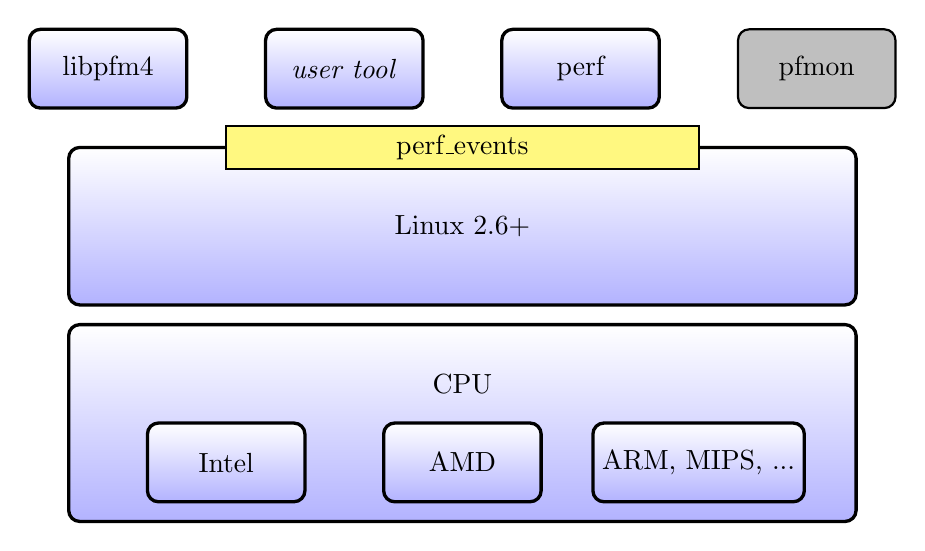
\begin{tikzpicture}[scale=1,transform shape]
\tikzstyle{size}=[minimum width=2 cm, minimum height=1 cm,anchor=center]

\tikzstyle{module}=[size,rectangle,rounded corners,draw=black, top color=white, bottom color=blue!30,very thick, text centered]
\tikzstyle{interface}=[rectangle,draw=black, fill=yellow!50,thick, text centered]
\tikzstyle{label}=[size,rectangle,text centered]

\node [module,minimum width=10 cm,minimum height=2.5 cm] at (0,0.5) (cpu)  {};
\node [label] at (0,1) (cpuLabel) {CPU};
\node [module] at (-3,0) (intel)  {Intel};
\node [module] at (0,0) (amd) {AMD};
\node [module] at (3,0) (arm) {ARM, MIPS, ...};

\node [module,minimum width=10 cm,minimum height=2 cm] at (0,3) (linux)  {Linux 2.6+};

\node [interface,minimum width=6 cm] at (0,4) (perf)  {perf\_events};

\node [module] at (-4.5,5) (libpfm4)  {libpfm4};
\node [module] at (-1.5,5) (user)  {\textit{user tool}};
\node [module] at (1.5,5) (perf)  {perf};
\node [size,rectangle,rounded corners,draw,thick,fill=gray!50] at (4.5,5) (pfmon)  {pfmon \Cross};

\end{tikzpicture}
